\section{Experimental setups}

\subsection{Key components}
\paragraph{Scintillation detector}
is used to detect ionizing radiation in general. Here we have gamma radiation. The purpose of scintillator is to lower photon energy via photoelectric effect, Compton scattering, and pair production~\cite{wermes}. It is then connected to photomultiplier tube (PMT) to generate signals.
\begin{figure}[ht]
   \centering
   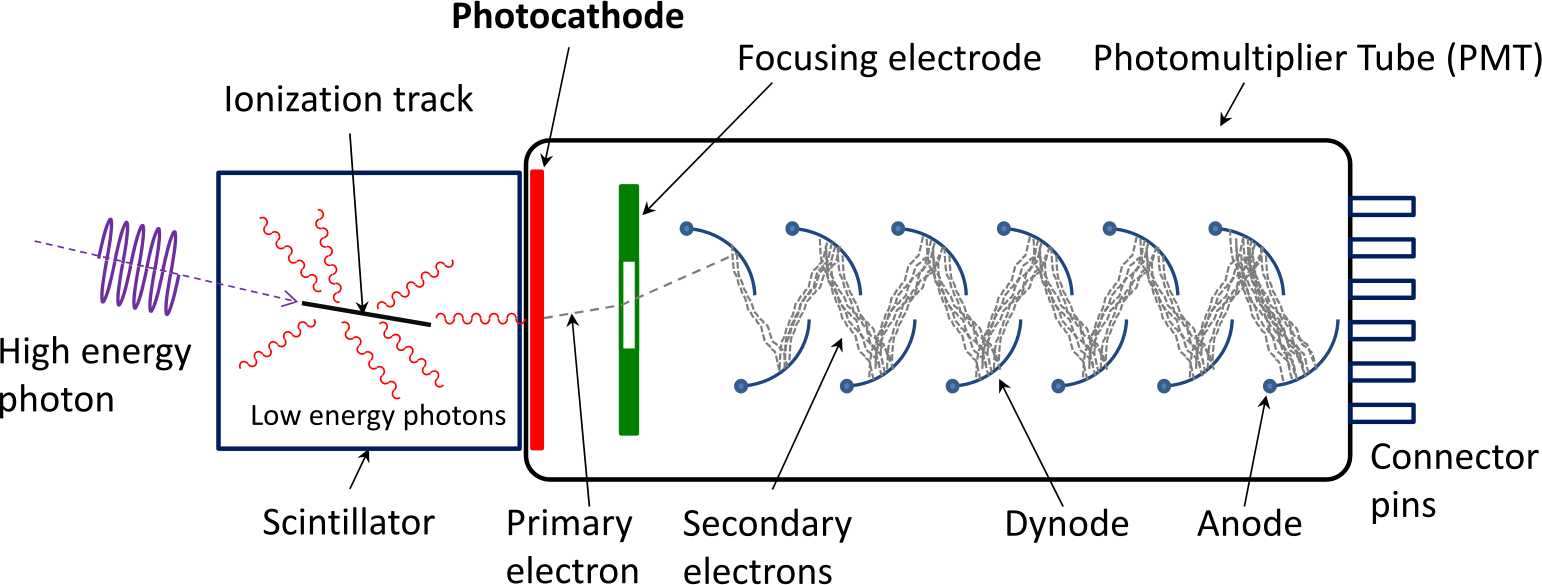
\includegraphics[width=0.9\linewidth]{Scintillator.png}
   \caption{Scintillator with PMT~\cite{wikiScin}}%
\end{figure}

\paragraph{Fast-slow coincidence} is the technique to measure the ionizing radiation separately. The "slow" part will determine the energy of incoming radiation. And the "fast" part is used to measure the time as precisely as possible, since the photomultiplier will be brought to saturation and the height of the pulse is not proportional to radiation energy any more~\cite{IACI1968103}. \textcolor{blue}{How exactly configure the fast and slow part? By adjusting the voltage?}

\paragraph{SCA} stands for single channel analyzer. Basically it is advanced version of simple discriminator, as one can set both upper-level (ULD) and lower-level discriminator (LLD) for SCA. It reads the input pulse and check whether it is within the preset limits or not. If it is, SCA will produce a uniform digital signal.
When applied to PMT, the height of pulse corresponds to energy of radiation. If SCA is built in after PMT, we are essentially picking out photons within the SCA window. Thus the name~\cite{SCAmanual}.

Simple discriminator outputs logic signal right after input goes higher than threshold. Since SCA also needs to check the ULD, it will produce output after maximal amplitude. There are two modes: non-timing and timing SCA. Non-timing SCA generates output right after the input comes back to the LLD, i.e.~after its peak. It will create the so-called "time walk" meaning that logic output will differ in time, even thought the inputs are simultaneous but of different height. Timing SCA, on the other hand, outputs logic signal as soon as the input hits its maximum~\cite{SCAmanual}.

%TODO: too much explanation, need to cut before hand in!

\paragraph{CFD} stands for constant fraction discriminator. As its name suggests, it gets triggered at some preset fraction of maximal amplitude, in order to reduce "walk". In simplest form, CFD works by splitting input signals, inverting one of them, and adding delay to the other. In the end, by combining these two together, we get logic signal with minimal walk~\cite{CFDmanual}.

%TODO: actually three parts, relating to comparator. Can adjust delay to cope with different rise time

\paragraph{TAC} stands for time-to-amplitude converter, which outputs pulse with amplitude proportional to time difference between start and end signals.

\paragraph{Time resolution} of fast coincidence unit is $< \SI{100}{\nano\s}$ on any single input and $< \SI{1}{\mu\s}$ on the coincidence output~\cite{fastmanual}.

\paragraph{Expected Spectrum} of ${}^{60} \text{Co}$ would predominantly consists of $\SI{0.31}{\mega\eV}$ $\beta$-line and \SI{1.1732}{\mega\eV}, \SI{1.3325}{\mega\eV} $\gamma$-line~\cite{firestone}. Its $\gamma$-spectrum can be found in~\ref{fig:CoSpec}, where one can see two clear peaks corresponding to the $\gamma$-radiations and some background because of various effects, like pair production (higher $E$), Compton scattering (mid $E$), and photoelectric effect (low $E$)~\cite{wermes}.

\begin{figure}[ht]
   \centering
   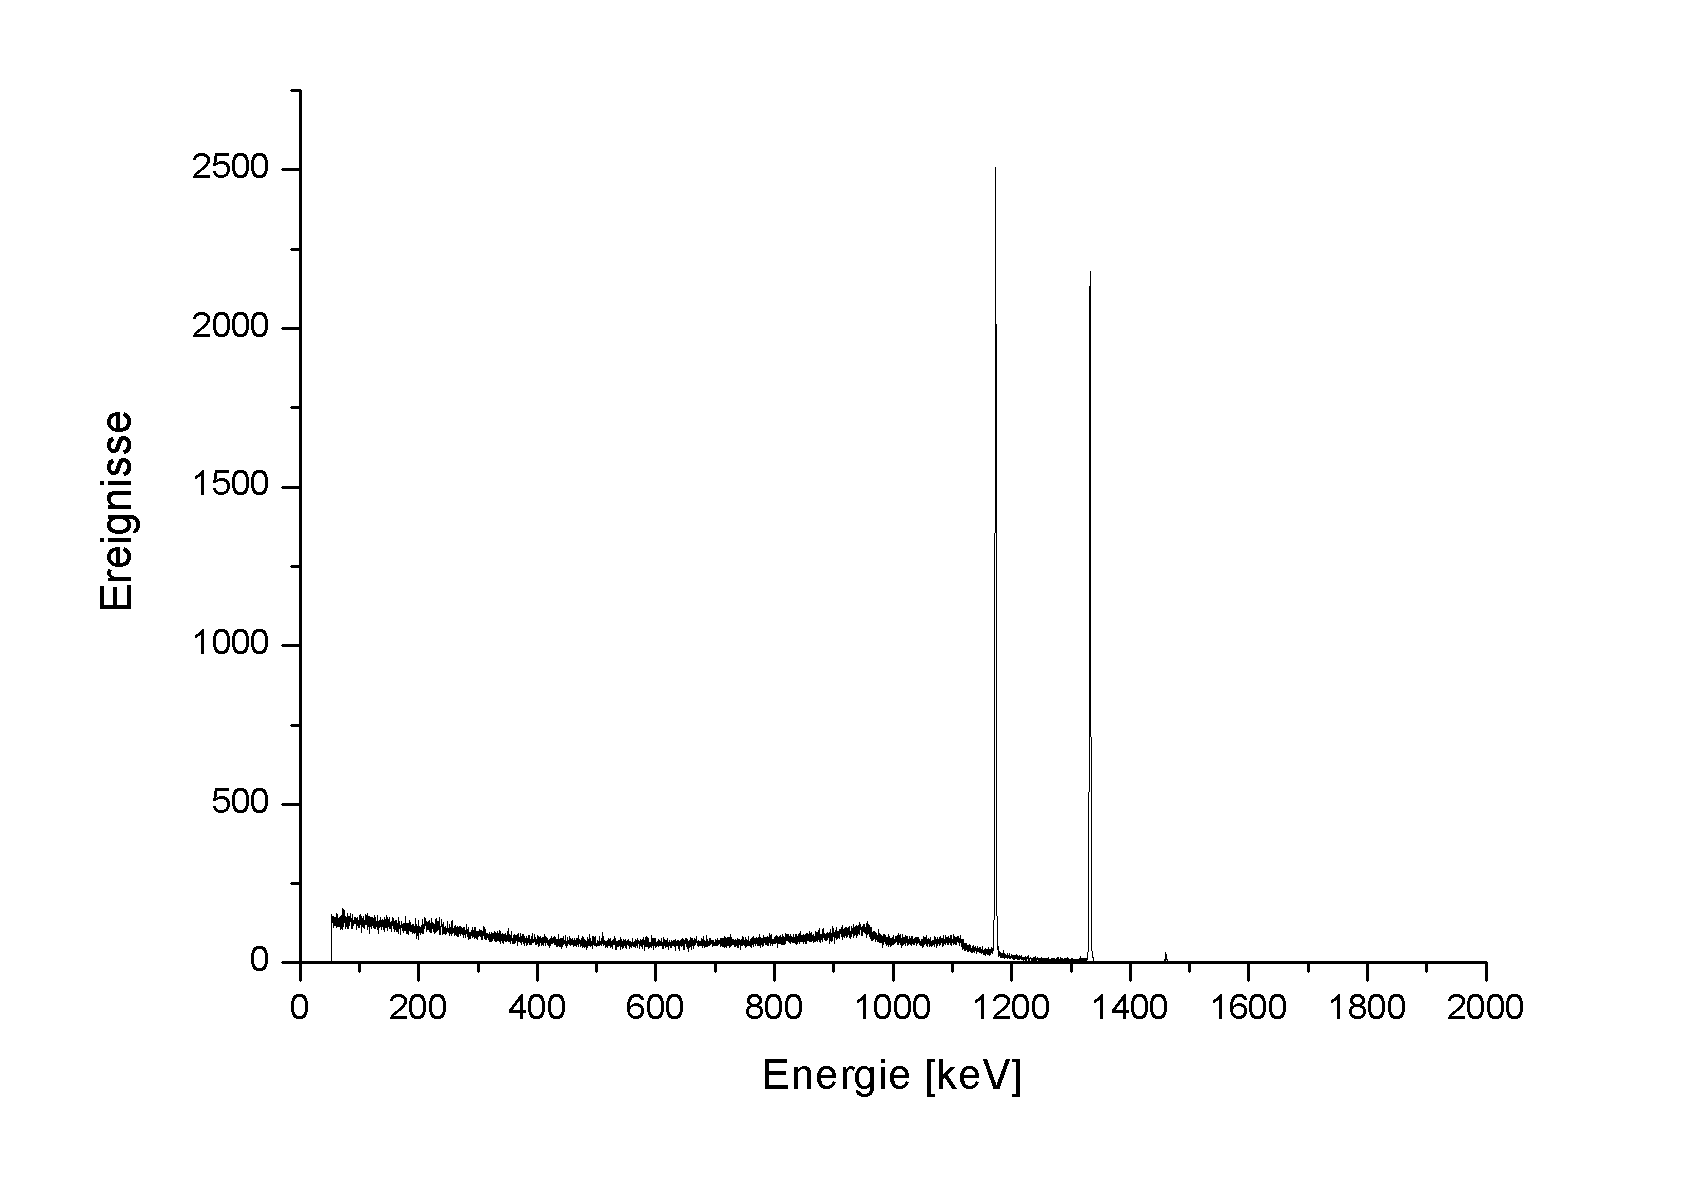
\includegraphics[width=0.8\linewidth]{60Co_gamma_spectrum_energy.png}
   \caption{${}^{60}\text{Co}$ $\gamma$-specturm~\cite{CoSpec}}%
   \label{fig:CoSpec}
\end{figure}
